% !TEX root =./main.tex

\section{Block 11: Tracking/Velocity Estimation - Csicsila}

\subsection{Tracking}
The tracking feature add quality to the sonar project. Using an 'X' crosshair, this stage successfully follows the most prominent object as it moves across the monitor. To achieve this, the \code{xcorr2} function was used. This function takes the signal and a template and then runs a Cross-correlation algorithm to find which part of the graph most closely matches the template. This is similar to convolution. Once that is complete, the maximum point of the correlation is found and indexed to get the row and col, to overlay the crosshair on the image. 

The template is comprised of a 4x4 array filled with 1's. This template was chosen with the target in mind. The target was essentially a blob with higher values toward the center. Therefore, the template would correlate with the highest in the middle of that blob. This template plan also worked for the second object that was much longer and thinner than the first object. This is because the middle of that object still had a concentration of higher values which matched with the template.

\begin{figure}[H]
    \centering
    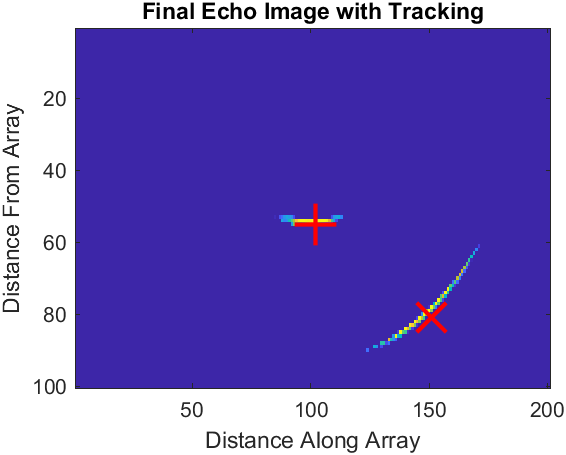
\includegraphics[width=0.5\linewidth]{figures/TrackingImage2.png}
    \caption{Final Echo Image with Tracking}
    \label{fig:TrackingImage2}
\end{figure}

Figure \ref{fig:TrackingImage2} shows the one frame where both objects are in sight with the crosshairs overlaid. The picture was colored to show the intensity around the blob better. This image also show cases the programs ability to detect two prominent images at once which will be discussed later on. 

\begin{figure}[H]
    \centering
    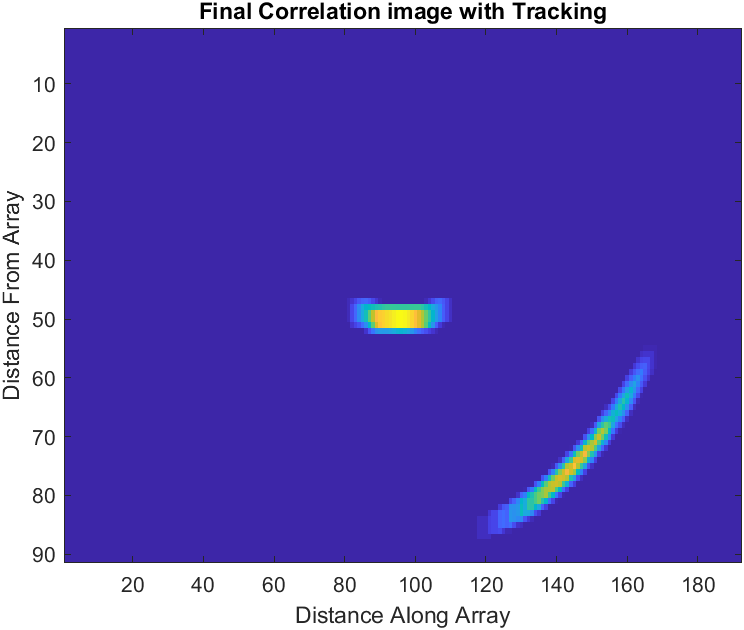
\includegraphics[width=0.5\linewidth]{figures/TrackingImage1.png}
    \caption{Final Correlation image with Tracking}
    \label{fig:TrackingImage1}
\end{figure}

Figure \ref{fig:TrackingImage1} looks very similar but shows the correlation between the template and the original signal. As you can see, the correlation made each signal thicker and more prominent. This allowed the function to better understand where the denser part of the blob was for tracking purposes.

Before testing with the live image, test data was made to ensure that it would perform correctly. The first test data utilized an array with multiple different hotspots of intensity/

\begin{figure}[H]
    \centering
    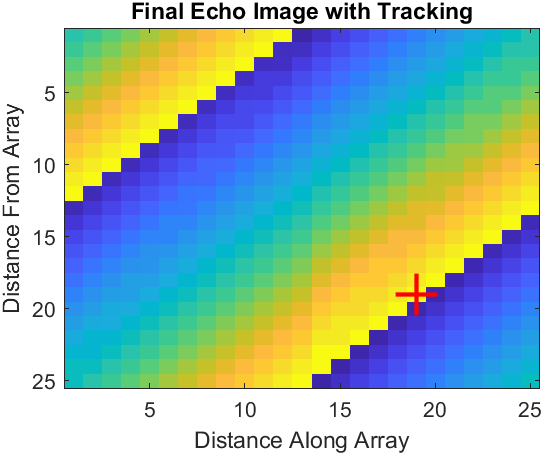
\includegraphics[width=0.5\linewidth]{figures/TrackingImage3.png}
    \caption{Test Image with Tracking}
    \label{fig:TrackingImage3}
\end{figure}

Figure \ref{fig:TrackingImage3} shows the random data with hotspots (highlighted by the lighter colors). Look what happens when the correlation with the same template is used.

\begin{figure}[H]
    \centering
    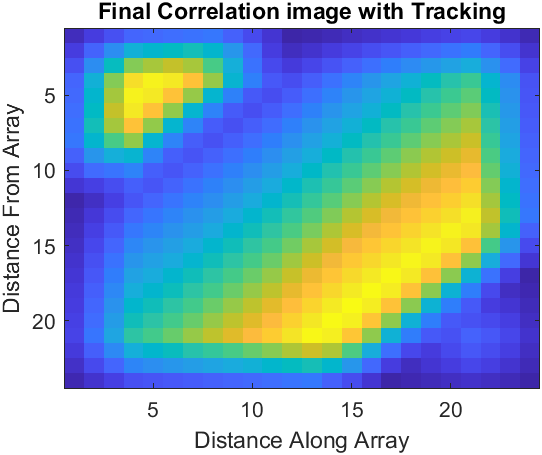
\includegraphics[width=0.5\linewidth]{figures/TrackingImage4.png}
    \caption{Test Image Correlation with Tracking}
    \label{fig:TrackingImage4}
\end{figure}

As seen in Figure \ref{fig:TrackingImage4}, the correlation was able to pick out the lower right corner as being more similar to the template. This mainly due to the lower pixel count of this image. Nevertheless, the program would work with the live image.

The next task was to try to implement tracking for two objects. This was a bit more challenging and had mild success with the live image. The problem trying to be solved was finding local maxima for the data. The first theoretical approach was to use derivatives, however this would be impractical and very slow for the size of this data. Therefore, another method was implemented. First, correlation was done in the same manner was the first tests. Then, an offset was used to zero out the values around the max value. This way, correlation could be done again without selecting the same point. 

\begin{figure}[H]
    \centering
    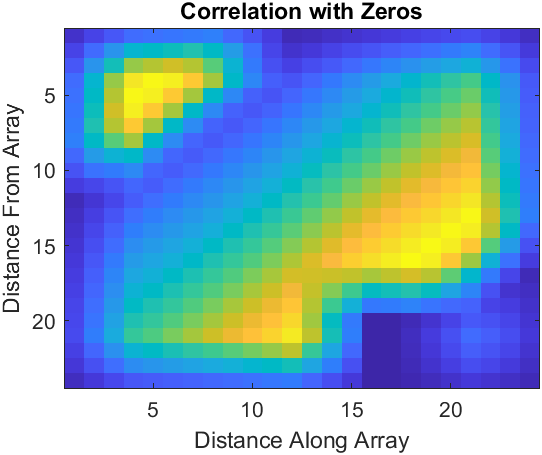
\includegraphics[width=0.5\linewidth]{figures/TrackingImage5.png}
    \caption{Test Image Correlation with Zeros}
    \label{fig:TrackingImage5}
\end{figure}

Figure \ref{fig:TrackingImage5} shows the correlation after the zeros are removed. Comparing this to \ref{fig:TrackingImage4}, there is clearly an empty spot. The zero offset could be increased to essential increase the radius in which to ignore objects around the original object.

However, an issue arose with edge cases. When setting the zeros with the offset it would sometimes set values outside the range of the array to 0 which would throw an error. To fix this, the edges of the scan were temporarily removed to avoid the error. Then the location was calculated then the edges were returned. This did not affect quality, and solved the issue.

\begin{figure}[H]
    \centering
    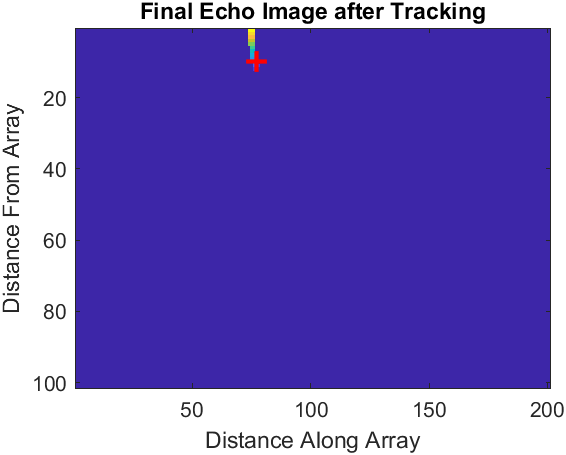
\includegraphics[width=0.5\linewidth]{figures/TrackingImage6.png}
    \caption{Image Correlation Edge Case}
    \label{fig:TrackingImage6}
\end{figure}

Figure \ref{fig:TrackingImage6} was created to test the edge cases so prove that the program could still detect images close to the edge.

\subsection{Velocity}

Velocity was extremely simple to produce. Because the tracking showed the location of the image, a simple distance equation could be used.

\begin{equation}
    d = \sqrt{(pixelPerFootRow(x_{2} - x_{1}))^{2} + pixelPerFootCol(y_{2} - y_{1})^{2}}
    \label{eq:distanceEQ}
\end{equation}

The last tricky part was figuring out the timing to get the velocity. Knowing that each scan consisted of 4000 samples, and the new up sampled sampling frequency was 200kHz, the time was found. The final step was choosing two tracked images to get the distance. An image a iteration 5 and 50 were chosen. Therefore, the final time had to be multiplied by 45 to account for the time difference between iteration.

The estimated velocity was around 2.4 ft/s.


